\thispagestyle{endchapter}

\begin{tcolorbox}

\vspace{80pt}
	\lettrine{T}{he} 2013 expedition drew to a close. The pushing had been harder, 
	and perhaps not as immediately rewarding as the previous year. The vast pitches and storming phreatic were 
	elusive in most areas. The one exception of course being the surprise find below \passage{Balamory}: the big
	active rift pitch series from \passage{Kokain} to \passage{Pick Your Poison}. But \passage{Minestrone} had 
	failed to yield to extensive pushing, \passage{Invictus} gave up with a terminal aven, \passage{Brezno Slapov}
	proved too wet to push far. 
	
	Despite this 1.8km of passage was found, at great depth. After a final push to \passage{Slinging in the Rain} 
	Rhys Tyers and Oliver Myerscough put the cave to sleep for the year, hauling out the 5 bags they managed to 
	pack \passage{X-Ray} into.
	
	The weather had been exceptionally good for the entire expedition and this was reflected in the general morale. 
	To take advantage of the good weather the expedition decamped the mountain a couple of days early to enjoy the 
	baking heat of \passage{Tolmin}, and the cooling waters of the \passage{So\v{c}a} river. The JSPDT and ICCC parted ways for the year.

	The longest cave in Slovenia would be waiting for them next year.

\end{tcolorbox} 
	\backgroundsetup{	scale=1,
					color=black,
					opacity=1,
					angle=0,
					contents={%
							  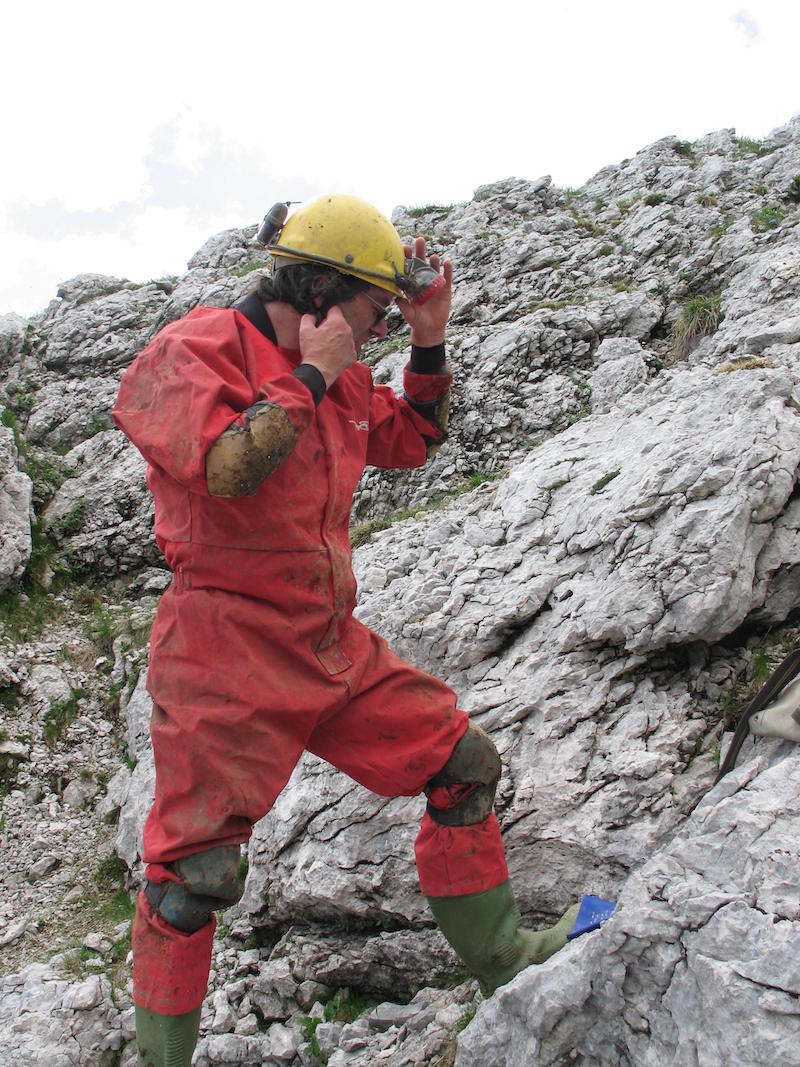
\includegraphics[height=\paperheight]{images/backgrounds/dave-2013.jpg}
 					}
	}
\BgThispage
